\documentclass[conference]{IEEEtran}
\IEEEoverridecommandlockouts
%\usepackage{cite}
\usepackage{amssymb,amsfonts}
\usepackage{bm}
\usepackage{amsmath}
\usepackage{algorithm}
\usepackage{algpseudocode}
\usepackage{graphicx}
\usepackage{textcomp}
\usepackage{xcolor}
\def\BibTeX{{\rm B\kern-.05em{\sc i\kern-.025em b}\kern-.08em
    T\kern-.1667em\lower.7ex\hbox{E}\kern-.125emX}}
% Custom personalization
\DeclareMathOperator*{\argmax}{arg\,max}
\DeclareMathOperator*{\argmin}{arg\,min}
\parskip 1ex
\parindent 0pt
\usepackage[spanish]{babel}
\usepackage{csquotes}
\usepackage{hyperref}
\usepackage[backend=biber,style=ieee]{biblatex}
\addbibresource{references.bib}

\begin{document}

\title{BATS: Bridging Acoustic Transparency in Speech}

\author{\IEEEauthorblockN{Diego Quezada}
\IEEEauthorblockA{\textit{Departamento de Informática} \\
\textit{Universidad Técnica Federico Santa María}\\
Valparaíso, Chile \\
diego.quezadac@sansano.usm.cl}
\and
\IEEEauthorblockN{Felipe Cisternas}
\IEEEauthorblockA{\textit{Departamento de Informática} \\
\textit{Universidad Técnica Federico Santa María}\\
Valparaíso, Chile \\
felipe.cisternasal@sansano.usm.cl}}

\maketitle

\begin{abstract}

El reconocimiento de voz se basa en representaciones de señales acústicas, como espectrogramas y MFCCs. Sin embargo, los modelos actuales son en gran medida opacos en cuanto a cómo toman decisiones en este proceso. La naturaleza física de los datos de entrada en el reconocimiento de voz agrega una capa adicional de complejidad, lo que plantea el desafío de mejorar la transparencia y la comprensión de estos modelos para garantizar un reconocimiento de voz más preciso y confiable.

\end{abstract}

\begin{IEEEkeywords}
ASR, XAI, CNN, RNN, Transformers
\end{IEEEkeywords}

\section{Introducción}

En el ámbito del reconocimiento de voz, la selección de un modelo y su arquitectura es fundamental para enfrentar los retos específicos que esta disciplina impone. Modelos de vanguardia como Whisper, que se basan en la arquitectura de Transformers de OpenAI, son altamente eficaces pero actúan como cajas negras, lo que significa que los procesos de decisión que siguen para convertir señales de audio en palabras no son transparentes. Esta falta de explicabilidad, esencial para generar confianza en los usuarios, hace imperativo el uso de técnicas de eXplainable Artificial Intelligence (XAI) para desentrañar y comprender cómo estos modelos avanzados toman sus decisiones.

La explicabilidad en modelos de reconocimiento de voz no solo mejora la comprensión del proceso de toma de decisiones, sino que también es clave para aumentar su robustez, especialmente cuando dichos modelos se integran como componentes centrales en un software. Esta característica se vuelve esencial para ganar la confianza de los usuarios en el producto final. Sin embargo, el desafío se intensifica debido a la naturaleza física y compleja de los datos de entrada, lo que dificulta proporcionar explicaciones claras y de alto nivel basadas en estos datos. Por ello, es crucial mantener un equilibrio entre avanzar en la precisión y eficiencia de los modelos y desarrollar soluciones que mejoren su explicabilidad, asegurando así un balance óptimo entre rendimiento y comprensión del modelo.

Esta investigación tiene como objetivo mejorar la comprensión de los modelos de reconocimiento de voz para que los usuarios, especialmente aquellos con discapacidades auditivas, puedan confiar en su funcionamiento.

\subsection{Trabajo relacionado}

La investigaciones sobre explicabilidad en modelos de reconocimiento de voz son escasas pero destacan por su aplicación innovadorea de métodos de explicabilidad.

En \cite{10094635} se aborda la tarea reconocimiento de voz utilizando el conjunto de datos CommonVoice \cite{commonvoice:2020} y tres sistemas de reconocimiento de voz: Google API, Sphinx y DeepSpeech. Los autores plantean las explicaciones como un subconjunto de fotogramas de audio que son causas mínimas y suficientes de la transcripción. Para esto, adaptan las técnicas de clasificación de imagen SFL \cite{sun2020explaining} y explicaciones composicionales \cite{unknown} para luego compararlas con las ofrecidas por LIME \cite{ribeiro2016why}.

En \cite{wu2023trust} se aborda la tarea de \textbf{reconocimiento de fonemas} utilizando el conjunto de datos TIMIT \cite{timit} y el método LIME junto a dos variantes propuestas: LIME-WS y LIME-TS. El conjunto de datos TIMIT segmenta los distintos fonemas en los datos de entrada. Los autores utilizan como representación interpretable un vector que indica la presencia o ausencia de cada segmento de audio. El objetivo es identificar los segmentos más importantes para la predicción del siguiente fonema. Inicialmente, para la generación del vecindario se aplican máscaras aleatorias a los segmentos de TIMIT. Luego, considerando que al analizar un fonema es probable que solo los segmentos cercanos incidan en su identificación, LIME-WS solo aplica máscaras aleatorias a segmentos cercanos al fonema analizado y mantiene los lejanos constantes. Finalmente, en LIME-TS se consideran segmentos creados por un intervalo de tiempo en vez de los definidos por TIMIT y se aplica la misma idea de localidad que en LIME-WS.

En \cite{DBLP:journals/corr/abs-2008-00582} se aborda la tarea de etiquetado de música. Los autores plantean la necesidad de dar \textbf{explicaciones audibles} y proponen audioLIME como una extensión de LIME que utiliza explicaciones basadas en separación de fuentes.

\section{Método propuesto}

\subsection{Marco teórico}

El reconocimiento de voz, o más conocido en inglés como \textit{speech recognition}, es la tarea de asignar una secuencia de palabras a señales acústicas que contienen lenguaje hablado. 
Implica reconocer las palabras pronunciadas en una grabación de audio y transcribirlas a un formato escrito. El objetivo es transcribir con precisión el discurso en tiempo real o a partir de audio grabado, teniendo en cuenta factores como el acento, la velocidad del habla y el ruido de fondo.
Cuando la transcripción se realiza en tiempo real se habla de reconocimiento automático de voz o \textit{Automatic Speech Recognition} (ASR) en inglés. Considerando $\mathbf{X} = (x^{(1)}, x^{(2)} ,\dots, x^{(T)})$ como una secuencia de audio de largo $T$ e $y = (y_1, y_2, \dots, y_N)$ como una secuencia de palabras de largo $N$ podemos definir la tarea de reconocimiento de voz de manera precisa mediante el siguiente problema de optimización:

\begin{equation}
    f^\ast(\mathbf{X}) = \argmax_{\mathbf{y}} P^\ast(\mathbf{y}| \mathbf{X} = X)
\end{equation}

Donde $P^\ast$ es la verdadera distribución de probabilidad condicional que relaciona las entradas $\mathbf{X}$ con las salidas $\mathbf{y}$ \cite{Goodfellow-et-al-2016}.

La representación utilizada para $\mathbf{X}$ es de vital importancia para el desempeño de un modelo de reconocimiento de voz. La representación más simple es mediante una serie temporal univariada que modela la amplitud de la \textbf{señal de audio} en el tiempo. Al dividir la señal de audio en pequeñas ventanas de tiempo y calculando el espectro de frecuencia para cada ventana se obtiene un \textbf{espectrograma}: una representación visual de la señal de audio en el tiempo y en el dominio de la frecuencia. A partir del espectrograma se pueden extraer características de audio tales como los \textbf{coeficientes cepstrales de Mel} (MFCCs) que son ampliamente utilizados en la literatura para el reconocimiento de voz.

LIME \cite{ribeiro2016why} es un modelo agnóstico que explica de manera local las predicciones de un modelo \textbf{caja negra} $f$ mediante la aproximación de $f$ con un modelo \textbf{explicable} $g$ en una vecindad de la instancia de interés $\bm{x}$. LIME utiliza una \textbf{representación interpretable} $\bm{x^\prime} \in \{0,1\}^{d^\prime}$ de la instancia $\bm{x} \in \mathbb{R}^d$. De esta forma, el dominio de la explicación $g$ es $\{0,1\}^{d^\prime}$ y, por lo tanto, $g$ actúa sobre la presencia o ausencia de \textit{componentes interpretables}. Para generar la vecindad se utiliza una función $\pi_x(z)$ que mide la distancia entre dos puntos $x$ y $z$ en el espacio de atributos interpretable. Adicionalmente, dado que la idea es aproximar $f$ mediante un modelo interpretable, se considera una penalización $\Omega$ que mide la complejidad de $g$. Finalmente, y considerando una función de pérdida $\mathcal{L}(f, g, \pi_x)$ que mide la imprecisión del modelo $g$ al aproximar $f$ en la vecindad de $\bm{x}$ de acuerdo a la función de distancia $\pi$, la explicación producida por LIME que asegura \textbf{interpretabilidad} y \textbf{fidelidad local} se obtiene según la siguiente fórmula:

\begin{equation}
    \xi(\bm{x}) = \argmin_{g \in G} \mathcal{L}(f, g, \pi_x) + \Omega(g).
\end{equation}

Donde $G$ es el conjunto de todos los modelos interpretables considerados, como por ejemplo modelos lineales o árboles de decisión.

El borrado de representaciones \cite{li2017understanding} es un método \textbf{post-hoc} y \textbf{modelo agnóstico}, que consiste en eliminar características del input y ver como varían las predicciones del modelo, para así determinar las características más importantes a la hora de predecir.
En esta investigación, analizaremos e interpretaremos las decisiones de un modelo de caja negra observando los efectos al borrar varias partes de la representación, en este caso como lo pueden ser las distintas dimensiones de los MFCCs. Sea $f$ un modelo neuronal de ASR, dado un ejemplo $e \in E$ con una transcripción $t$, calcularemos el score de una métrica $M$ con la siguiente fórmula:
\begin{equation}
    S_{M}(e,t) = M(t, f(e))
\end{equation}
Ahora sea $d$ una dimensión de nuestro vector $e$ la cual queremos explorar, denotaremos $S_{M}(e,t,\neg d)$ el score cuando la dimensión $d$ es removida; esto quiere decir que todos sus valores son 0.
La importancia de la dimensión $d$ denotada por $I(d)$ estará dada por la diferencia relativa entre $S_{M}(e,t)$ y $S_{M}(e,t,\neg d)$:
\begin{equation} \label{eq:imp}
    I(d) = \frac{1}{|E|} \sum_{e \in E} \frac{S_{M}(e,t) - S_{M}(e,t,\neg d)}{S_{M}(e,t)}
\end{equation}
Para esto utilizaremos métricas ampliamente utilizadas al evaluar tareas de Automatic Speech Recognition (ASR) como lo son:
\begin{itemize}
    \item Word Error Rate (WER)
    \item Match Error Rate (MER)
    \item Word Information Lost (WIL)
    \item Word Information Preserved (WIP)
    \item Character Error Rate (CER)
\end{itemize}
Y calcularemos la importancia de cada dimensión con cada métrica dada la diferencia relativa entre los outputs del modelo.

\subsection{Conjunto de datos}

En la presente investigación se utilizará el conjunto de datos \href{https://commonvoice.mozilla.org/en/datasets}{\textit{CommonVoice}} \cite{commonvoice:2020}. En particular, se utilizarán las grabaciones en inglés asociadas a la versión 11 de CommonVoice disponible en HuggingFace Datasets.

Los conjunto de entrenamiento, validación y prueba consisten en 948736, 16354 y 16354 grabaciones de audio respectivamente. Cada grabación de audio tiene asociada una transcripción. Adicionalmente, cada grabación de audio fue grabada con un \textit{sampling rate} de 48 kHz.

\subsection{Descripción propuesta}

La propuesta busca evaluar la explicabilidad de modelos estado del arte en la tarea de reconocimiento de voz mediante métodos \textbf{post-hoc}.

\subsubsection{SLIME}

Para explicar las transcripciones del modelo Whisper, se propone el algoritmo \textbf{SLIME} (Speech LIME) que modela cómo diferentes modificaciones en la señal de audio afectan la calidad de la transcripción.

SLIME fragmenta una grabación de audio en segmentos de 100 milisegundos y considera como representación interpretable un vector booleano que indica la presencia o ausencia de cada segmento. Utilizando esta representación, se genera una vecindad de 100 instancias apagando segmentos de manera aleatoria. Cada instancia de la vecindad fue transcrita por Whisper, y mediante la distancia de Levenshtein entre la transcripción perturbada y la original se cuantificó el impacto de los silencios, proporcionando una base para una comparación cuantitativa entre las transcripciones. Finalmente, se ajustó un modelo explicable de regresión lineal considerando la representación interpretable de los audios como entrada y la distancia de Levenshtein como salida, lo cual permitió evaluar la importancia de los segmentos.

Debido a la alta demanda computacional que implica obtener predicciones de Whisper, se limitó la vecindad exploratoria a 100 combinaciones. Esto estableció un equilibrio entre la profundidad del análisis y las restricciones prácticas.

Los coeficientes resultantes de la regresión lineal ofrecen una interpretación directa de la relevancia de cada segmento de audio. Los segmentos asociados con coeficientes negativos son clave; su presencia es vital para mantener la fidelidad de la transcripción original, mientras que su ausencia es indicativa de un incremento en la distancia de Levenshtein, reflejando transcripciones que se desvían de la original. Esta información es útil para discernir las partes del audio que el modelo considera importantes para una transcripción precisa. El siguiente paso es mejorar la segmentación del audio, buscando métodos que puedan captar con mayor precisión las unidades lingüísticas significativas y mejorar la interpretación de las decisiones del modelo.

En \ref{alg:slime} se resume el algoritmo propuesto para obtener las explicaciones de Whisper mediante LIME.

\begin{algorithm}
\caption{SLIME}
\begin{algorithmic}[1]
\State $S \gets \emptyset$
\State $f \gets$ Black-box model
\State $n$ $\gets$ Number of segments of 100 ms in audio
\State $x \gets$ Original audio instance
\State $y \gets f(x)$
\State $x' \gets$ Vector of $n$ ones
\State $P \gets$ Generate 100 Binomial perturbations of $x'$
\For{each $p$ in $P$}
    \State $z \gets$ Apply $p$ to $x$
    \State $d \gets$  Levenshtein distance between $y$ and $f(z)$
    \State $z' \gets$ Apply random mask to $x'$
    \State $S \gets S \cup (z', d)$
\EndFor
\State $g \gets$ Fit linear model to $S$
\State \textbf{end algorithm}
\end{algorithmic}
\label{alg:slime}
\end{algorithm}


\section{Resultados preliminares}

\subsection{SLIME}

Consideremos una grabación de audio $x$ cuyo contenido es \textit{they perfectly illuminate the flowerbeds of gardens}. Al aplicar SLIME a esta grabación se obtiene la explicación de la Figura \ref{fig:slime}.

\begin{figure}[H]
\centerline{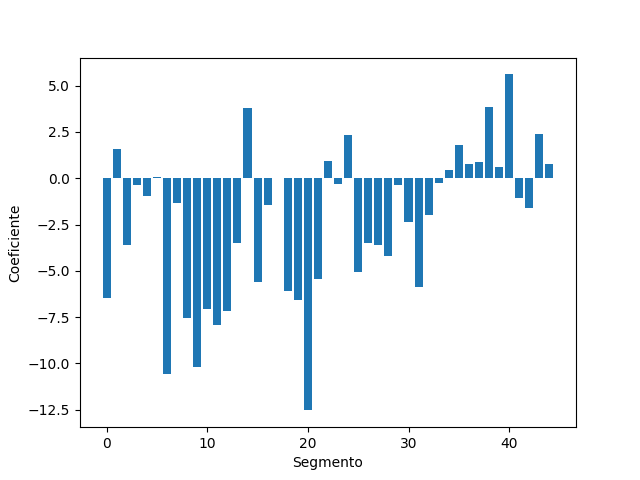
\includegraphics[width=0.5\textwidth]{./images/slime.png}}
\caption{Explicación de SLIME}
\label{fig:slime}
\end{figure}

Como se mencionó anteriormente, un coeficiente negativo indican que un segmento es importante pues al removerlo la transcripción se desvía de la original considerando la distancia de Levenshtein.

\subsubsection{Borrado de representaciones}

\subsection{Importancia Common Voice 11}
\begin{figure}[H]
\centering
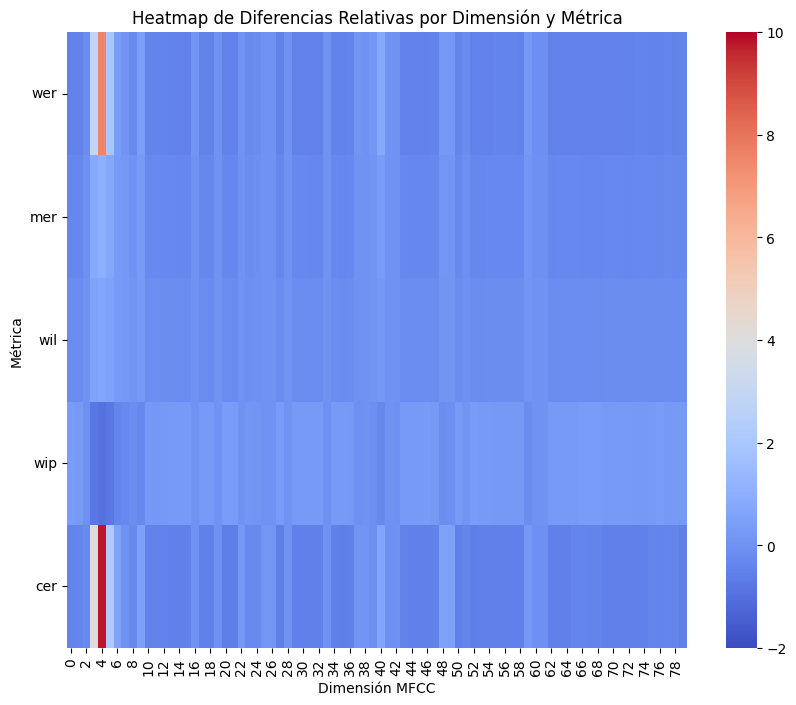
\includegraphics[width=0.5\textwidth]{images/importance_plot.png}
\caption{Mapa de calor de iImportancias $I(d)$ calculado usando la eEcuación \ref{eq:imp}. Cada celda muestra la importancia de una dimensión (columna) de losl MFCCs en cada métrica (fila) para el modelo entrenado.}
\end{figure}

\printbibliography
\end{document}